\documentclass[11pt]{article}
\usepackage[a4paper,margin=2.5cm]{geometry}
\usepackage{amsmath,graphicx,booktabs,multirow,subcaption,rotating,wrapfig,longtable,siunitx,tikz,pgfplots}
\pgfplotsset{compat=1.17}
\title{Stress Test Three: Figures and Tables}
\author{D. Drawing}
\date{}
\begin{document}
\maketitle
\section{Pictures}
A photograph-like raster image comes first. It is followed by a TikZ diagram with labels, a pgfplots chart,
and a grid of four panels. The text between them must stay in order.

\begin{figure}[h]
\centering
\includegraphics[width=0.5\textwidth]{photo.png}
\caption{A raster image with a gradient.}
\end{figure}

\begin{wrapfigure}{r}{0.35\textwidth}
\centering
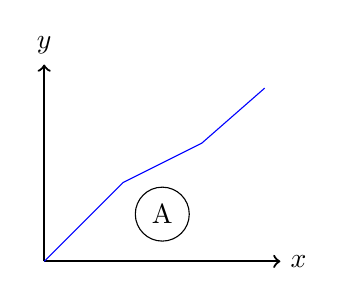
\begin{tikzpicture}
\draw[thick,->] (0,0) -- (3,0) node[right] {$x$};
\draw[thick,->] (0,0) -- (0,2.5) node[above] {$y$};
\draw[blue] (0,0) -- (1,1) -- (2,1.5) -- (2.8,2.2);
\node[draw,circle] at (1.5,0.6) {A};
\end{tikzpicture}
\caption{A TikZ sketch next to text.}
\end{wrapfigure}
This paragraph wraps around a small figure placed at the right margin. Wrapped figures are awkward because
the lines of text beside them are shorter than usual, and a converter could mistake the figure's labels
for part of the paragraph. We therefore write several sentences here, so that the paragraph is clearly
longer than the figure is tall, and the text continues below the figure at full width again. The labels
$x$ and $y$ and the letter A in the circle belong to the figure and should not be read as text.

\begin{figure}[h]
\centering
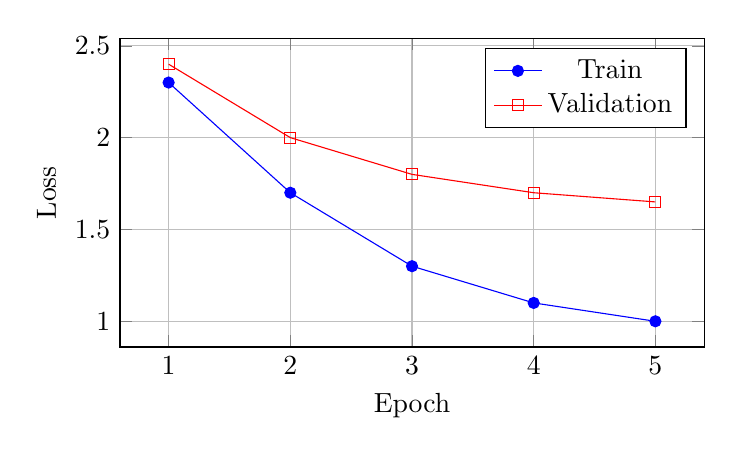
\begin{tikzpicture}
\begin{axis}[width=9cm,height=5.5cm,xlabel={Epoch},ylabel={Loss},legend pos=north east,grid=major]
\addplot[mark=*,blue] coordinates {(1,2.3) (2,1.7) (3,1.3) (4,1.1) (5,1.0)};
\addplot[mark=square,red] coordinates {(1,2.4) (2,2.0) (3,1.8) (4,1.7) (5,1.65)};
\legend{Train,Validation}
\end{axis}
\end{tikzpicture}
\caption{A vector chart drawn by pgfplots, with a legend and grid lines.}
\end{figure}

\begin{figure}[h]
\centering
\begin{subfigure}{0.45\textwidth}\includegraphics[width=\linewidth]{lines.pdf}\caption{Signals}\end{subfigure}\hfill
\begin{subfigure}{0.45\textwidth}\includegraphics[width=\linewidth]{bars.pdf}\caption{Counts}\end{subfigure}\\[1em]
\begin{subfigure}{0.45\textwidth}\includegraphics[width=\linewidth]{scatter.pdf}\caption{Points}\end{subfigure}\hfill
\begin{subfigure}{0.45\textwidth}\includegraphics[width=\linewidth]{heat.pdf}\caption{Heat}\end{subfigure}
\caption{A two by two grid of panels (a)--(d).}
\end{figure}

\section{Tables}
Table~\ref{tab:math} has formulas in its cells; Table~\ref{tab:wide} is wide.

\begin{table}[h]
\centering
\caption{Formulas in cells.}\label{tab:math}
\begin{tabular}{lcc}
\toprule
Function & Derivative & Integral \\
\midrule
$x^n$ & $n x^{n-1}$ & $\frac{x^{n+1}}{n+1}$ \\
$e^{x}$ & $e^{x}$ & $e^{x}$ \\
$\sin x$ & $\cos x$ & $-\cos x$ \\
$\ln x$ & $1/x$ & $x\ln x - x$ \\
\bottomrule
\end{tabular}
\end{table}

\begin{table}[h]
\centering
\small
\caption{A wide table with twelve columns.}\label{tab:wide}
\begin{tabular}{lrrrrrrrrrrr}
\toprule
City & Jan & Feb & Mar & Apr & May & Jun & Jul & Aug & Sep & Oct & Nov \\
\midrule
Amsterdam & 3.4 & 3.8 & 6.3 & 9.2 & 13.1 & 15.6 & 17.9 & 17.5 & 14.5 & 10.7 & 6.7 \\
Brussels & 3.3 & 3.7 & 6.8 & 9.8 & 13.6 & 16.2 & 18.4 & 18.0 & 14.9 & 11.1 & 6.8 \\
Paris & 5.0 & 5.6 & 8.8 & 11.4 & 15.1 & 18.2 & 20.4 & 20.2 & 16.9 & 13.0 & 8.4 \\
Rome & 7.5 & 8.2 & 10.8 & 13.3 & 17.7 & 21.7 & 24.4 & 24.4 & 20.9 & 16.4 & 11.7 \\
\bottomrule
\end{tabular}
\end{table}

\begin{table}[h]
\centering
\caption{Merged header cells and a grid.}
\begin{tabular}{|c|c|c|c|}
\hline
\multirow{2}{*}{Group} & \multicolumn{3}{c|}{Score} \\ \cline{2-4}
 & Low & Mid & High \\ \hline
A & 12 & 30 & 8 \\ \hline
B & 9 & 41 & 15 \\ \hline
\end{tabular}
\end{table}

A borderless table, as often found in reports:

\begin{center}
\begin{tabular}{lll}
Name & Role & Office \\
Anna & Editor & 2.14 \\
Bram & Reviewer & 3.02 \\
Chen & Author & 1.07 \\
\end{tabular}
\end{center}

\begin{sidewaystable}
\centering
\caption{A rotated table.}
\begin{tabular}{llll}
\toprule
Model & Data & Metric & Score \\
\midrule
Alpha & Set 1 & F1 & 0.81 \\
Beta & Set 2 & F1 & 0.77 \\
\bottomrule
\end{tabular}
\end{sidewaystable}

\begin{longtable}{rll}
\caption{A table that runs over a page break.}\\
\toprule
No. & Item & Note \\
\midrule
\endfirsthead
\toprule
No. & Item & Note \\
\midrule
\endhead
\bottomrule
\endfoot
1 & Apples & fresh \\ 2 & Pears & ripe \\ 3 & Plums & sour \\ 4 & Grapes & sweet \\ 5 & Figs & dried \\
6 & Dates & soft \\ 7 & Limes & green \\ 8 & Kiwis & hairy \\ 9 & Mango & large \\ 10 & Melon & heavy \\
11 & Cherries & red \\ 12 & Peach & fuzzy \\ 13 & Lemon & sour \\ 14 & Berry & small \\ 15 & Guava & pink \\
16 & Papaya & long \\ 17 & Quince & hard \\ 18 & Olive & salty \\ 19 & Apricot & orange \\ 20 & Lychee & white \\
21 & Coconut & brown \\ 22 & Banana & yellow \\ 23 & Orange & round \\ 24 & Tomato & red \\ 25 & Pepper & hot \\
26 & Carrot & long \\ 27 & Onion & strong \\ 28 & Garlic & strong \\ 29 & Leek & mild \\ 30 & Kale & bitter \\
\end{longtable}
The document ends after the long table with this sentence.
\end{document}
